\section{Finger Knuckle Project}
\subsection{Using histogram equalization to normalize image}
I have tried linear, log, and histogram to normalize image for getting better bounding box detection. From experiments, I found histogram equalization algorithm can get the best performance for detecting finger knuckle on the dark light.


\begin{figure}[ht!]
    \centering
    \subfloat[]{
        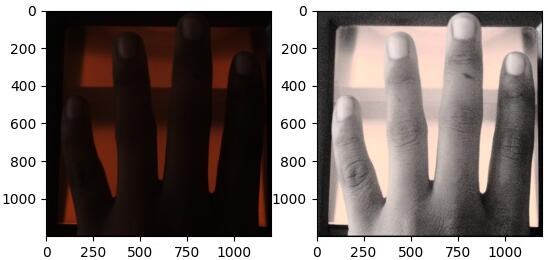
\includegraphics[width=3in]{Figure/18-11-2022/histogram_1.jpg}
        \label{}
    }
    \subfloat[]{
        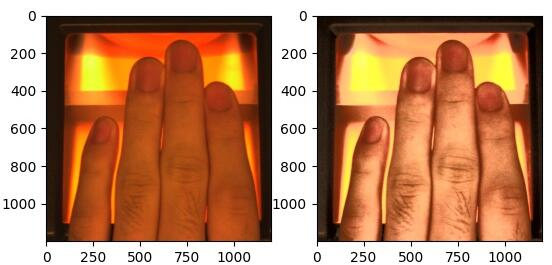
\includegraphics[width=3in]{Figure/18-11-2022/histogram_2.jpg}
        \label{}
    }

    \subfloat[]{
        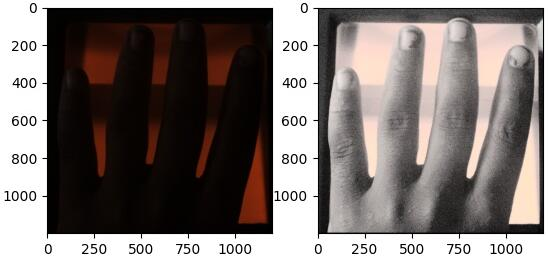
\includegraphics[width=3in]{Figure/18-11-2022/histogram_3.jpg}
        \label{}
    }
    \subfloat[]{
        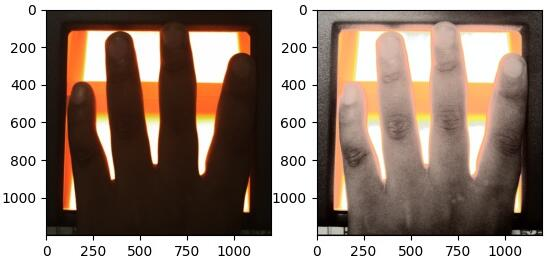
\includegraphics[width=3in]{Figure/18-11-2022/histogram_4.jpg}
        \label{}
    }

    \caption{After using histogram equalization algorithm, the texture of finger knuckle is very clear for detecting.}
    \label{histogram}
\end{figure}

\subsection{Choose the hyperparameters}
\subsubsection{Input image size}
I have tried that change the input image size $h\times w$ from $128\times128$ to $208\times184$. As for the former size, it just follows the RFN model parameter, and the latter input image size is the mean size of the segmented finger knuckle. When I train the RFN model, I also removed the values of ten pixels on each side of the finger knuckle for eliminating background interference. I just used the RFN to test the performance on the middle finger knuckle of left hand, as shown the 